\documentclass[11pt,fleqn, openany]{book} % Default font size and left-justified equations

%%%%%%%%%%%%%%%%%%%%%%%%%%%%%%%%%%%%%%%%%
% The Legrand Orange Book
% Structural Definitions File
% Version 2.1 (26/09/2018)
%
% Original author:
% Mathias Legrand (legrand.mathias@gmail.com) with modifications by:
% Vel (vel@latextemplates.com)
% 
% This file was downloaded from:
% http://www.LaTeXTemplates.com
%
% License:
% CC BY-NC-SA 3.0 (http://creativecommons.org/licenses/by-nc-sa/3.0/)
%
%%%%%%%%%%%%%%%%%%%%%%%%%%%%%%%%%%%%%%%%%

%----------------------------------------------------------------------------------------
%	VARIOUS REQUIRED PACKAGES AND CONFIGURATIONS
%----------------------------------------------------------------------------------------

\usepackage[table]{xcolor}

\usepackage{graphicx}
\usepackage{tabularx} % Required for including pictures
\usepackage{pgf,tikz,tkz-tab,eurosym,yhmath, stmaryrd}
\usepackage{pgfplots}
\usepackage{mathrsfs}
\usetikzlibrary{patterns}
\usetikzlibrary{trees}
\graphicspath{{../../Pictures/}}
\usepackage{multicol} 


\usepackage[english]{babel} % English language/hyphenation
\usepackage{icomma}
\usepackage{enumitem} % Customize lists
\setlist{nolistsep, nosep, nolistsep} % Reduce spacing between bullet points and numbered lists

\usepackage{booktabs} % Required for nicer horizontal rules in tables

 % Required for specifying colors by name


\definecolor{ocre}{RGB}{243,102,25} % Define the orange color used for highlighting throughout the book

\usepackage{listings}

\definecolor{codegreen}{rgb}{0,0.6,0}
\definecolor{codegray}{rgb}{0.5,0.5,0.5}
\definecolor{codepurple}{rgb}{0.58,0,0.82}
\definecolor{backcolour}{rgb}{0.95,0.95,0.92}

\lstdefinestyle{mystyle}{
    backgroundcolor=\color{backcolour},   
    commentstyle=\color{codegreen},
    keywordstyle=\color{magenta},
    numberstyle=\tiny\color{codegray},
    stringstyle=\color{codepurple},
    basicstyle=\ttfamily\footnotesize,
    breakatwhitespace=false,         
    breaklines=true,                 
    captionpos=b,                    
    keepspaces=true,                 
    numbers=left,                    
    numbersep=5pt,                  
    showspaces=false,                
    showstringspaces=false,
    showtabs=false,                  
    tabsize=2
}

\lstset{style=mystyle}

%----------------------------------------------------------------------------------------
% Paramétrage XSIM
%----------------------------------------------------------------------------------------

\usepackage[no-files]{xsim}


\DeclareExerciseEnvironmentTemplate{myex}{%
    \textbf{%
      \hypertarget{ex:\ExerciseID}{\sffamily{\ensuremath{\blacktriangleright}} Exercice \GetExerciseProperty{counter} \GetExerciseProperty{subtitle} --}
      \hyperlink{sol:\ExerciseID}{Voir le corrigé}%
    }\par
}{\par\smallskip}

\DeclareExerciseEnvironmentTemplate{mysol}{%
    \textbf{%
      \hypertarget{sol:\ExerciseID}{\sffamily{\ensuremath{\blacktriangleright}} Correction \GetExerciseProperty{counter} --}
      \hyperlink{ex:\ExerciseID}{Voir l'énoncé}%
    }\par
}{\par\medskip}

\xsimsetup{
  exercise/template = myex ,
  solution/template = mysol 
}

%Collection exercices

\DeclareExerciseTagging{topic}

\xsimsetup{collect}

%----------------------------------------------------------------------------------------
% SYMBOLES
%----------------------------------------------------------------------------------------

\newcommand\imCMsym[4][\mathord]{%
  \DeclareFontFamily{U} {#2}{}
  \DeclareFontShape{U}{#2}{m}{n}{
    <-6> #25
    <6-7> #26
    <7-8> #27
    <8-9> #28
    <9-10> #29
    <10-12> #210
    <12-> #212}{}
  \DeclareSymbolFont{CM#2} {U} {#2}{m}{n}
  \DeclareMathSymbol{#4}{#1}{CM#2}{#3}
}
\newcommand\alsoimCMsym[4][\mathord]{\DeclareMathSymbol{#4}{#1}{CM#2}{#3}}

\imCMsym{cmmi}{124}{\CMjmath}

\newcommand{\Oij}{(O\,;\,\vec{\imath}\,,\, \vec{\CMjmath} )}
\newcommand{\Oijk}{(O\,;\,\vec{\imath}\,,\, \vec{\CMjmath}\,,\,\vec{k})}

\newcommand\e{\mathrm{e}}
\newcommand\R{\mathbb{R}}
\newcommand\N{\mathbb{N}}


%----------------------------------------------------------------------------------------
%	MARGINS
%----------------------------------------------------------------------------------------

\usepackage{geometry} % Required for adjusting page dimensions and margins

\geometry{
	paper=a4paper, % Paper size, change to letterpaper for US letter size
	top=3cm, % Top margin
	bottom=3cm, % Bottom margin
	left=2cm, % Left margin
	right=2cm, % Right margin
	headheight=14pt, % Header height
	footskip=1.4cm, % Space from the bottom margin to the baseline of the footer
	headsep=10pt, % Space from the top margin to the baseline of the header
	%showframe, % Uncomment to show how the type block is set on the page
}

\setlength{\parindent}{0pt}
\parskip=5pt



%----------------------------------------------------------------------------------------
%	FONTS
%----------------------------------------------------------------------------------------

\usepackage{avant} % Use the Avantgarde font for headings
\usepackage{times} % Use the Times font for headings
\usepackage{mathptmx} % Use the Adobe Times Roman as the default text font together with math symbols from the Sym­bol, Chancery and Com­puter Modern fonts

%\usepackage{microtype} % Slightly tweak font spacing for aesthetics
%\usepackage[utf8]{inputenc} % Required for including letters with accents
\usepackage[T1]{fontenc} % Use 8-bit encoding that has 256 glyphs

%----------------------------------------------------------------------------------------
%	BIBLIOGRAPHY AND INDEX
%----------------------------------------------------------------------------------------

\usepackage[style=numeric,citestyle=numeric,sorting=nyt,sortcites=true,autopunct=true,babel=hyphen,hyperref=true,abbreviate=false,backref=true,backend=biber]{biblatex}
\addbibresource{bibliography.bib} % BibTeX bibliography file
\defbibheading{bibempty}{}

\usepackage{calc} % For simpler calculation - used for spacing the index letter headings correctly
\usepackage{makeidx} % Required to make an index
\makeindex % Tells LaTeX to create the files required for indexing

%----------------------------------------------------------------------------------------
%	MAIN TABLE OF CONTENTS
%----------------------------------------------------------------------------------------

\usepackage{titletoc} % Required for manipulating the table of contents

\contentsmargin{0cm} % Removes the default margin

% Part text styling (this is mostly taken care of in the PART HEADINGS section of this file)
\titlecontents{part}
	[0cm] % Left indentation
	{\addvspace{20pt}\bfseries} % Spacing and font options for parts
	{}
	{}
	{}

% Chapter text styling
\titlecontents{chapter}
	[1.25cm] % Left indentation
	{\addvspace{12pt}\large\sffamily\bfseries} % Spacing and font options for chapters
	{\color{ocre!60}\contentslabel[\Large\thecontentslabel]{1.25cm}\color{ocre}} % Formatting of numbered sections of this type
	{\color{ocre}} % Formatting of numberless sections of this type
	{\color{ocre!60}\normalsize\;\titlerule*[.5pc]{.}\;\thecontentspage} % Formatting of the filler to the right of the heading and the page number

% Section text styling
\titlecontents{section}
	[1.25cm] % Left indentation
	{\addvspace{3pt}\sffamily\bfseries} % Spacing and font options for sections
	{\contentslabel[\thecontentslabel]{1.25cm}} % Formatting of numbered sections of this type
	{} % Formatting of numberless sections of this type
	{\hfill\color{black}\thecontentspage} % Formatting of the filler to the right of the heading and the page number

% Subsection text styling
\titlecontents{subsection}
	[1.25cm] % Left indentation
	{\addvspace{1pt}\sffamily\small} % Spacing and font options for subsections
	{\contentslabel[\thecontentslabel]{1.25cm}} % Formatting of numbered sections of this type
	{} % Formatting of numberless sections of this type
	{\ \titlerule*[.5pc]{.}\;\thecontentspage} % Formatting of the filler to the right of the heading and the page number

% Figure text styling
\titlecontents{figure}
	[1.25cm] % Left indentation
	{\addvspace{1pt}\sffamily\small} % Spacing and font options for figures
	{\thecontentslabel\hspace*{1em}} % Formatting of numbered sections of this type
	{} % Formatting of numberless sections of this type
	{\ \titlerule*[.5pc]{.}\;\thecontentspage} % Formatting of the filler to the right of the heading and the page number

% Table text styling
\titlecontents{table}
	[1.25cm] % Left indentation
	{\addvspace{1pt}\sffamily\small} % Spacing and font options for tables
	{\thecontentslabel\hspace*{1em}} % Formatting of numbered sections of this type
	{} % Formatting of numberless sections of this type
	{\ \titlerule*[.5pc]{.}\;\thecontentspage} % Formatting of the filler to the right of the heading and the page number

%----------------------------------------------------------------------------------------
%	MINI TABLE OF CONTENTS IN PART HEADS
%----------------------------------------------------------------------------------------

% Chapter text styling
\titlecontents{lchapter}
	[0em] % Left indentation
	{\addvspace{15pt}\large\sffamily\bfseries} % Spacing and font options for chapters
	{\color{ocre}\contentslabel[\Large\thecontentslabel]{1.25cm}\color{ocre}} % Chapter number
	{}  
	{\color{ocre}\normalsize\sffamily\bfseries\;\titlerule*[.5pc]{.}\;\thecontentspage} % Page number

% Section text styling
\titlecontents{lsection}
	[0em] % Left indentation
	{\sffamily\small} % Spacing and font options for sections
	{\contentslabel[\thecontentslabel]{1.25cm}} % Section number
	{}
	{}

% Subsection text styling (note these aren't shown by default, display them by searchings this file for tocdepth and reading the commented text)
\titlecontents{lsubsection}
	[.5em] % Left indentation
	{\sffamily\footnotesize} % Spacing and font options for subsections
	{\contentslabel[\thecontentslabel]{1.25cm}}
	{}
	{}

%----------------------------------------------------------------------------------------
%	HEADERS AND FOOTERS
%----------------------------------------------------------------------------------------


\usepackage{fancyhdr} % Required for header and footer configuration

\pagestyle{fancy}
\renewcommand{\chaptermark}[1]{\markboth{\sffamily\normalsize\bfseries\ \thechapter.\ #1}{}} % Chapter text font settings
\renewcommand{\sectionmark}[1]{\markright{\sffamily\normalsize\thesection\hspace{5pt}#1}{}} % Section text font settings
\fancyhf{} \fancyhead[LE,RO]{\sffamily\normalsize\thepage} % Font setting for the page number in the header
\fancyhead[LO]{\rightmark} % Print the nearest section name on the left side of odd pages
\fancyhead[RE]{\leftmark} % Print the current chapter name on the right side of even pages

\fancyfoot[L]{Jason LAPEYRONNIE}
\fancyfoot[R]{\href{http://mathoutils.fr}{http://mathoutils.fr}} % Uncomment to include a footer

\renewcommand{\headrulewidth}{0.5pt} % Thickness of the rule under the header
\renewcommand{\footrulewidth}{0.5pt} % Thickness of the rule under the header

\fancypagestyle{plain}{% Style for when a plain pagestyle is specified
	\fancyhead{}\renewcommand{\headrulewidth}{0pt}%
}

% Removes the header from odd empty pages at the end of chapters
\makeatletter
\renewcommand{\cleardoublepage}{
\clearpage\ifodd\c@page\else
\hbox{}
\vspace*{\fill}
\thispagestyle{empty}
\newpage
\fi}

%----------------------------------------------------------------------------------------
%	THEOREM STYLES
%----------------------------------------------------------------------------------------

\usepackage{amsmath,amsfonts,amssymb,amsthm} % For math equations, theorems, symbols, etc

\newcommand{\intoo}[2]{\mathopen{]}#1\,;#2\mathclose{[}}
\newcommand{\ud}{\mathop{\mathrm{{}d}}\mathopen{}}
\newcommand{\intff}[2]{\mathopen{[}#1\,;#2\mathclose{]}}
\renewcommand{\qedsymbol}{$\blacksquare$}
\newtheorem{notation}{Notation}[section]

% Boxed/framed environments
\newtheoremstyle{ocrenumbox}% Theorem style name
{0pt}% Space above
{0pt}% Space below
{\normalfont}% Body font
{}% Indent amount
{\small\bf\sffamily\color{ocre}}% Theorem head font
{\;:\;}% Punctuation after theorem head
{0.25em}% Space after theorem head
{\small\sffamily\color{ocre}\thmname{#1}\nobreakspace\thmnumber{\@ifnotempty{#1}{}\@upn{#2}}% Theorem text (e.g. Theorem 2.1)
\thmnote{\nobreakspace\the\thm@notefont\sffamily\bfseries\color{black}---\nobreakspace#3}} % Optional theorem note

\newtheoremstyle{blacknumex}% Theorem style name
{5pt}% Space above
{10pt}% Space below
{\normalfont}% Body font
{} % Indent amount
{\small\bf\sffamily}% Theorem head font
{\;:\;}% Punctuation after theorem head
{0.25em}% Space after theorem head
{\small\sffamily{\tiny\ensuremath{\blacksquare}}\nobreakspace\thmname{#1}\nobreakspace\thmnumber{\@ifnotempty{#1}{}\@upn{#2}}% Theorem text (e.g. Theorem 2.1)
\thmnote{\nobreakspace\the\thm@notefont\sffamily\bfseries---\nobreakspace#3}}% Optional theorem note

\newtheoremstyle{blacknumexo}% Theorem style name
{15pt}% Space above
{10pt}% Space below
{\normalfont}% Body font
{} % Indent amount
{\small\bf\sffamily}% Theorem head font
{}% Punctuation after theorem head
{0.5em}% Space after theorem head
{\small\sffamily{\ensuremath{\blacktriangleright}}\nobreakspace\thmname{#1}\nobreakspace\thmnumber{\@ifnotempty{#1}{}\@upn{#2}}% Theorem text (e.g. Theorem 2.1)
\thmnote{\nobreakspace\the\thm@notefont\sffamily\bfseries---\nobreakspace#3} \\}% Optional theorem note



\newtheoremstyle{blacknumbox} % Theorem style name
{0pt}% Space above
{5pt}% Space below
{}% Body font
{}% Indent amount
{\large\bf\sffamily}% Theorem head font
{\;:\;}% Punctuation after theorem head
{0.25em}% Space after theorem head
{\small\sffamily\thmname{#1}\nobreakspace\thmnumber{\@ifnotempty{#1}{}\@upn{#2}}% Theorem text (e.g. Theorem 2.1)
\thmnote{\nobreakspace\the\thm@notefont\sffamily\bfseries---\nobreakspace#3}}% Optional theorem note

% Non-boxed/non-framed environments
\newtheoremstyle{ocrenum}% Theorem style name
{5pt}% Space above
{5pt}% Space below
{\normalfont}% Body font
{}% Indent amount
{\small\bf\sffamily\color{ocre}}% Theorem head font
{\;:\;}% Punctuation after theorem head
{0.25em}% Space after theorem head
{\small\sffamily\color{ocre}\thmname{#1}\nobreakspace\thmnumber{\@ifnotempty{#1}{}\@upn{#2}}% Theorem text (e.g. Theorem 2.1)
\thmnote{\nobreakspace\the\thm@notefont\sffamily\bfseries\color{black}---\nobreakspace#3}} % Optional theorem note
\makeatother

% Defines the theorem text style for each type of theorem to one of the three styles above
\newcounter{dummy} 
\newcounter{thm}
\newcounter{correction}
\newcounter{qst}
\theoremstyle{ocrenumbox}
\newtheorem{theoremeT}[dummy]{Théorème}
\newtheorem{exerciseT}{Propriété}
\newtheorem{principeT}{Principe}
\theoremstyle{blacknumex}
\newtheorem{exampleT}{Exemple}
\theoremstyle{blacknumexo}
\newtheorem{exo}[thm]{Exercice}
\newtheorem{corr}[correction]{Correction}
\newtheorem{quest}[qst]{Question}
\theoremstyle{blacknumbox}
\newtheorem{vocabulary}{Vocabulary}[section]
\newtheorem{definitionT}{Définition}
\newtheorem{corollaryT}[dummy]{Corollary}
\theoremstyle{ocrenum}
\newtheorem{proofT}[dummy]{Démonstration}


%----------------------------------------------------------------------------------------
%	DEFINITION OF COLORED BOXES
%----------------------------------------------------------------------------------------

\RequirePackage[framemethod=default]{mdframed} % Required for creating the theorem, definition, exercise and corollary boxes

% Theorem box
\newmdenv[skipabove=7pt,
skipbelow=7pt,
backgroundcolor=black!5,
linecolor=ocre,
innerleftmargin=5pt,
innerrightmargin=5pt,
innertopmargin=10pt,
leftmargin=0cm,
rightmargin=0cm,
innerbottommargin=5pt]{tBox}

%Proposition box	  
\newmdenv[skipabove=7pt,
skipbelow=7pt,
rightline=false,
leftline=true,
topline=false,
bottomline=false,
backgroundcolor=ocre!10,
linecolor=ocre,
innerleftmargin=5pt,
innerrightmargin=5pt,
innertopmargin=10pt,
innerbottommargin=3pt,
leftmargin=0cm,
rightmargin=0cm,
linewidth=4pt]{eBox}	

% Definition box
\newmdenv[skipabove=7pt,
backgroundcolor=ocre!4,
skipbelow=7pt,
rightline=false,
leftline=true,
topline=false,
bottomline=false,
linecolor=ocre,
innerleftmargin=5pt,
innerrightmargin=5pt,
innertopmargin=10pt,
leftmargin=0cm,
rightmargin=0cm,
linewidth=4pt,
innerbottommargin=5pt]{dBox}	

% Corollary box
\newmdenv[skipabove=7pt,
skipbelow=7pt,
rightline=false,
leftline=true,
topline=false,
bottomline=false,
linecolor=gray,
backgroundcolor=black!5,
innerleftmargin=5pt,
innerrightmargin=5pt,
innertopmargin=5pt,
leftmargin=0cm,
rightmargin=0cm,
linewidth=4pt,
innerbottommargin=5pt]{cBox}

\newmdenv[skipabove=7pt,
skipbelow=7pt,
backgroundcolor=black!5,
innerleftmargin=5pt,
topline=false,
bottomline=false,
rightline=false,
leftline=false,
innerrightmargin=5pt,
innertopmargin=5pt,
leftmargin=0cm,
rightmargin=0cm,
innerbottommargin=5pt]{xBox}

% Creates an environment for each type of theorem and assigns it a theorem text style from the "Theorem Styles" section above and a colored box from above
\newenvironment{theorem}{\begin{tBox}\begin{theoremeT}}{\end{theoremeT}\end{tBox}}

\newenvironment{exo2}{\noindent \begin{exo}\item\relax \noindent \begin{eBox}\item\relax}{\end{eBox}\end{exo}}


\newenvironment{proposition}{\begin{eBox}\begin{exerciseT}}{\hfill{\color{ocre}}\end{exerciseT}\end{eBox}}		

\newenvironment{principe}{\begin{eBox}\begin{principeT}}{\hfill{\color{ocre}}\end{principeT}\end{eBox}}	
		  
\newenvironment{definition}{\begin{dBox}\begin{definitionT}}{\end{definitionT}\end{dBox}}	

\newenvironment{example}{\begin{xBox}\begin{exampleT}}{\hfill{\tiny\ensuremath{\blacksquare}}\end{exampleT}\end{xBox}}

\newenvironment{demonstration}{\begin{proofT}}{\hfill{\tiny\ensuremath{\square}}\end{proofT}}		
\newenvironment{corollary}{\begin{cBox}\begin{corollaryT}}{\end{corollaryT}\end{cBox}}	

%----------------------------------------------------------------------------------------
%	REMARK ENVIRONMENT
%----------------------------------------------------------------------------------------

\newenvironment{remark}{\par\vspace{5pt}\small % Vertical white space above the remark and smaller font size
\begin{list}{}{
\leftmargin=25pt % Indentation on the left
\rightmargin=15pt}\item\ignorespaces % Indentation on the right
\makebox[-2.5pt]{
\begin{tikzpicture}[overlay]
\node[draw=ocre!60,line width=1pt,circle,fill=ocre!25,font=\sffamily\bfseries,inner sep=2pt,outer sep=0pt] at (-15pt,0pt){\textcolor{ocre}{R}};\end{tikzpicture}} % Orange R in a circle
\advance\baselineskip -1pt}{\end{list}\vskip5pt} % Tighter line spacing and white space after remark

%----------------------------------------------------------------------------------------
%	SECTION NUMBERING IN THE MARGIN
%----------------------------------------------------------------------------------------

\makeatletter
\renewcommand{\@seccntformat}[1]{\llap{\textcolor{ocre}{\csname the#1\endcsname}\hspace{1em}}}                    
\renewcommand{\section}{\@startsection{section}{1}{\z@}
{-4ex \@plus -1ex \@minus -.4ex}
{1ex \@plus.2ex }
{\normalfont\LARGE\sffamily\bfseries}}
\renewcommand{\subsection}{\@startsection {subsection}{2}{\z@}
{-3ex \@plus -0.1ex \@minus -.4ex}
{0.5ex \@plus.2ex }
{\normalfont\sffamily\bfseries}}
\renewcommand{\subsubsection}{\@startsection {subsubsection}{3}{\z@}
{-2ex \@plus -0.1ex \@minus -.2ex}
{.2ex \@plus.2ex }
{\normalfont\small\sffamily\bfseries}}                        
\renewcommand\paragraph{\@startsection{paragraph}{4}{\z@}
{-2ex \@plus-.2ex \@minus .2ex}
{.1ex}
{\normalfont\small\sffamily\bfseries}}

%----------------------------------------------------------------------------------------
%	PART HEADINGS
%----------------------------------------------------------------------------------------

% Numbered part in the table of contents
\newcommand{\@mypartnumtocformat}[2]{%
	\setlength\fboxsep{0pt}%
	\noindent\colorbox{ocre!20}{\strut\parbox[c][.7cm]{\ecart}{\color{ocre!70}\Large\sffamily\bfseries\centering#1}}\hskip\esp\colorbox{ocre!40}{\strut\parbox[c][.7cm]{\linewidth-\ecart-\esp}{\Large\sffamily\centering#2}}%
}

% Unnumbered part in the table of contents
\newcommand{\@myparttocformat}[1]{%
	\setlength\fboxsep{0pt}%
	\noindent\colorbox{ocre!40}{\strut\parbox[c][.7cm]{\linewidth}{\Large\sffamily\centering#1}}%
}

\newlength\esp
\setlength\esp{4pt}
\newlength\ecart
\setlength\ecart{1.2cm-\esp}
\newcommand{\thepartimage}{}%
\newcommand{\partimage}[1]{\renewcommand{\thepartimage}{#1}}%
\def\@part[#1]#2{%
\ifnum \c@secnumdepth >-2\relax%
\refstepcounter{part}%
\addcontentsline{toc}{part}{\texorpdfstring{\protect\@mypartnumtocformat{\thepart}{#1}}{\partname~\thepart\ ---\ #1}}
\else%
\addcontentsline{toc}{part}{\texorpdfstring{\protect\@myparttocformat{#1}}{#1}}%
\fi%
\startcontents%
\markboth{}{}%
{\thispagestyle{empty}%
\begin{tikzpicture}[remember picture,overlay]%
\node at (current page.north west){\begin{tikzpicture}[remember picture,overlay]%	
\fill[ocre!20](0cm,0cm) rectangle (\paperwidth,-\paperheight);
\node[anchor=north] at (4cm,-3.25cm){\color{ocre!40}\fontsize{220}{100}\sffamily\bfseries\thepart}; 
\node[anchor=south east] at (\paperwidth-1cm,-\paperheight+1cm){\parbox[t][][t]{8.5cm}{
\printcontents{l}{0}{\setcounter{tocdepth}{1}}% The depth to which the Part mini table of contents displays headings; 0 for chapters only, 1 for chapters and sections and 2 for chapters, sections and subsections
}};
\node[anchor=north east] at (\paperwidth-1.5cm,-3.25cm){\parbox[t][][t]{15cm}{\strut\raggedleft\color{white}\fontsize{30}{30}\sffamily\bfseries#2}};
\end{tikzpicture}};
\end{tikzpicture}}%
\@endpart}
\def\@spart#1{%
\startcontents%
\phantomsection
{\thispagestyle{empty}%
\begin{tikzpicture}[remember picture,overlay]%
\node at (current page.north west){\begin{tikzpicture}[remember picture,overlay]%	
\fill[ocre!20](0cm,0cm) rectangle (\paperwidth,-\paperheight);
\node[anchor=north east] at (\paperwidth-1.5cm,-3.25cm){\parbox[t][][t]{15cm}{\strut\raggedleft\color{white}\fontsize{30}{30}\sffamily\bfseries#1}};
\end{tikzpicture}};
\end{tikzpicture}}
\addcontentsline{toc}{part}{\texorpdfstring{%
\setlength\fboxsep{0pt}%
\noindent\protect\colorbox{ocre!40}{\strut\protect\parbox[c][.7cm]{\linewidth}{\Large\sffamily\protect\centering #1\quad\mbox{}}}}{#1}}%
\@endpart}
\def\@endpart{\vfil\newpage
\if@twoside
\if@openright
\null
\thispagestyle{empty}%
\newpage
\fi
\fi
\if@tempswa
\twocolumn
\fi}

%----------------------------------------------------------------------------------------
%	CHAPTER HEADINGS
%----------------------------------------------------------------------------------------

% A switch to conditionally include a picture, implemented by Christian Hupfer
\newif\ifusechapterimage
\usechapterimagetrue
\newcommand{\thechapterimage}{}%
\newcommand{\chapterimage}[1]{\ifusechapterimage\renewcommand{\thechapterimage}{#1}\fi}%
\newcommand{\autodot}{.}
\def\@makechapterhead#1{%
{\parindent \z@ \raggedright \normalfont
\ifnum \c@secnumdepth >\m@ne
\if@mainmatter
\begin{tikzpicture}[remember picture,overlay]
\node at (current page.north west)
{\begin{tikzpicture}[remember picture,overlay]
\node[anchor=north west,inner sep=0pt] at (0,0) {\ifusechapterimage\includegraphics[width=\paperwidth]{\thechapterimage}\fi};
\draw[anchor=west] (\Gm@lmargin,-3cm) node [line width=2pt,rounded corners=15pt,draw=ocre,fill=white,fill opacity=0.5,inner sep=15pt]{\strut\makebox[22cm]{}};
\draw[anchor=west] (\Gm@lmargin+.3cm,-3cm) node {\huge\sffamily\bfseries\color{black}\thechapter\autodot~#1\strut};
\end{tikzpicture}};
\end{tikzpicture}
\else
\begin{tikzpicture}[remember picture,overlay]
\node at (current page.north west)
{\begin{tikzpicture}[remember picture,overlay]
\node[anchor=north west,inner sep=0pt] at (0,0) {\ifusechapterimage\includegraphics[width=\paperwidth]{\thechapterimage}\fi};
\draw[anchor=west] (\Gm@lmargin,-3cm) node [line width=2pt,rounded corners=15pt,draw=ocre,fill=white,fill opacity=0.5,inner sep=15pt]{\strut\makebox[22cm]{}};
\draw[anchor=west] (\Gm@lmargin+.3cm,-3cm) node {\huge\sffamily\bfseries\color{black}#1\strut};
\end{tikzpicture}};
\end{tikzpicture}
\fi\fi\par\vspace*{50\p@}}}

%-------------------------------------------

\def\@makeschapterhead#1{%
\begin{tikzpicture}[remember picture,overlay]
\node at (current page.north west)
{\begin{tikzpicture}[remember picture,overlay]
\node[anchor=north west,inner sep=0pt] at (0,0) {\ifusechapterimage\includegraphics[width=\paperwidth]{\thechapterimage}\fi};
\draw[anchor=west] (\Gm@lmargin,-3cm) node [line width=2pt,rounded corners=15pt,draw=ocre,fill=white,fill opacity=0.5,inner sep=15pt]{\strut\makebox[22cm]{}};
\draw[anchor=west] (\Gm@lmargin+.3cm,-3cm) node {\huge\sffamily\bfseries\color{black}#1\strut};
\end{tikzpicture}};
\end{tikzpicture}
\par\vspace*{50\p@}}
\makeatother

%----------------------------------------------------------------------------------------
%	LINKS
%----------------------------------------------------------------------------------------

\usepackage{hyperref}
\hypersetup{hidelinks,backref=true,pagebackref=true,hyperindex=true,colorlinks=false,breaklinks=true,urlcolor=ocre,bookmarks=true,bookmarksopen=false}

\usepackage{bookmark}
\bookmarksetup{
open,
numbered,
addtohook={%
\ifnum\bookmarkget{level}=0 % chapter
\bookmarksetup{bold}%
\fi
\ifnum\bookmarkget{level}=-1 % part
\bookmarksetup{color=ocre,bold}%
\fi
}
}

\renewcommand*\thesection{\arabic{section}}

\newcommand*{\coord}[3]{% 
  \ensuremath{\overrightarrow{#1}\, 
    \begin{pmatrix} 
      #2\\ 
      #3 
    \end{pmatrix}}}
    
  \newcommand*{\coordb}[2]{% 
  \ensuremath{ 
    \begin{pmatrix} 
      #1\\ 
      #2 
    \end{pmatrix}}}

\newcommand*{\coorde}[4]{% 
  \renewcommand{\arraystretch}{1}\ensuremath{\overrightarrow{#1}\, 
    \begin{pmatrix} 
      #2\\ 
      #3 \\
      #4
    \end{pmatrix}}}    
  \newcommand*{\coordbe}[3]{% 
 \renewcommand{\arraystretch}{1} \ensuremath{ 
    \begin{pmatrix} 
      #1\\ 
      #2 \\
      #3
    \end{pmatrix}}}  
    
\newcommand{\Card}{\mathrm{Card}}



\begin{document}

\chapterimage{../../Pictures/background}


\chapter{Cours : Convexité}



\section{Convexité, concavité}

\begin{definition}Soit $f$ une fonction définie sur un intervalle $I$. On note $\mathcal{C}_f$ la courbe représentative de $f$ dans un repère $\Oij$.
\begin{itemize}
\item On dit que $f$ est \textit{convexe} sur $I$ si, \textbf{pour tous réels} $a$ et $b$ dans $I$, avec $a<b$, la sécante reliant les deux points de la courbe d'abscisses $a$ et $b$ se trouve au-dessus de la courbe $\mathcal{C}_f$ sur $[a,b]$.
\item On dit que $f$ est \textit{concave} sur $I$ si,  \textbf{pour tous réels} $a$ et $b$ dans $I$, avec $a<b$, la sécante reliant les deux points de la courbe d'abscisses $a$ et $b$ se trouve en-dessous de la courbe $\mathcal{C}_f$ sur $[a,b]$.
\end{itemize}\end{definition}



\begin{minipage}{0.45\linewidth}
\begin{center}
\textbf{Fonction convexe}
\end{center}
\begin{center}
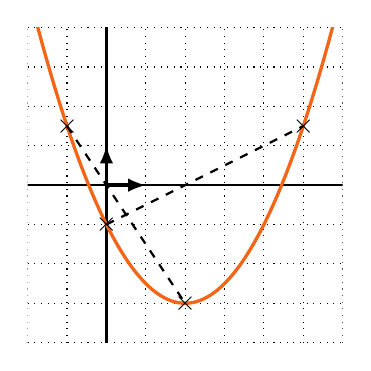
\begin{tikzpicture}[scale=0.5]
\clip (-2,-4) rectangle (6,4);
\draw [ thin, dotted] (-2,-4) grid (6,4);
\draw [thick] (-4,0)--(7,0);
\draw [thick] (0,-4) -- (0,5);
\draw [very thick,->,>=latex] (0,0)--(0,1);
\draw [very thick,->,>=latex] (0,0)--(1,0);
\draw [very thick, ocre,domain=-3:6,samples=100] plot (\x,{\x*\x/2-2*\x-1});
\draw [thick, dashed] (0,-1) -- (5,1.5);
\draw (0,-1) node {$\times$};
\draw (5,1.5) node {$\times$};
\draw [thick, dashed] (-1,1.5) -- (2,-3);
\draw (2,-3) node {$\times$};
\draw (-1,1.5) node {$\times$};
\end{tikzpicture}
\end{center}
\end{minipage}\hfill \begin{minipage}{0.45\linewidth}
\begin{center}
\textbf{Fonction concave}
\end{center}
\begin{center}
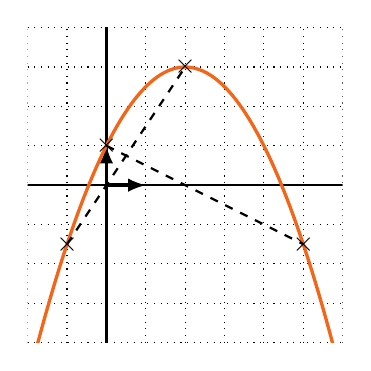
\begin{tikzpicture}[scale=0.5]
\clip (-2,-4) rectangle (6,4);
\draw [thin, dotted] (-2,-4) grid (6,4);
\draw [thick] (-4,0)--(7,0);
\draw [thick] (0,-4) -- (0,5);
\draw [very thick,->,>=latex] (0,0)--(0,1);
\draw [very thick,->,>=latex] (0,0)--(1,0);
\draw [very thick, ocre,domain=-3:6,samples=100] plot (\x,{-(\x*\x/2-2*\x-1)});
\draw [thick, dashed] (0,1) -- (5,-1.5);
\draw (0,1) node {$\times$};
\draw (5,-1.5) node {$\times$};
\draw [thick, dashed] (-1,-1.5) -- (2,3);
\draw (2,3) node {$\times$};
\draw (-1,-1.5) node {$\times$};
\end{tikzpicture}
\end{center}
\end{minipage}






\vskip10pt
\textbf{Rappel de certaines courbes représentatives}
\vskip5pt
\begin{minipage}{0.3\linewidth}
\begin{center}
\textbf{$x \mapsto x^2$}
\end{center}
\begin{center}
\begin{tikzpicture}[scale=0.65]
\clip (-3,-2) rectangle (3,3);
\draw [thick] (-4,0)--(7,0);
\draw [thick] (0,-4) -- (0,5);
\draw [very thick,->,>=latex] (0,0)--(0,1);
\draw [very thick,->,>=latex] (0,0)--(1,0);
\end{tikzpicture}
\end{center}
\end{minipage}\hfill\begin{minipage}{0.3\linewidth}

\begin{center}
\textbf{$x \mapsto \dfrac{1}{x}$}
\end{center}
\begin{center}
\begin{tikzpicture}[scale=0.65]
\clip (-3,-2) rectangle (3,3);
\draw [thick] (-4,0)--(7,0);
\draw [thick] (0,-4) -- (0,5);
\draw [very thick,->,>=latex] (0,0)--(0,1);
\draw [very thick,->,>=latex] (0,0)--(1,0);

\end{tikzpicture}
\end{center}
\end{minipage}\hfill\begin{minipage}{0.3\linewidth}
\begin{center}
\textbf{$x \mapsto x^3$}
\end{center}
\begin{center}
\begin{tikzpicture}[scale=0.65]
\clip (-3,-2) rectangle (3,3);
\draw [thick] (-4,0)--(7,0);
\draw [thick] (0,-4) -- (0,5);
\draw [very thick,->,>=latex] (0,0)--(0,1);
\draw [very thick,->,>=latex] (0,0)--(1,0);
\end{tikzpicture}
\end{center}
\end{minipage}

\begin{minipage}{0.3\linewidth}
\begin{center}
\textbf{$x \mapsto \ln(x)$}
\end{center}
\begin{center}
\begin{tikzpicture}[scale=0.65]
\clip (-3,-2) rectangle (3,2);
\draw [thick] (-4,0)--(7,0);
\draw [thick] (0,-4) -- (0,5);
\draw [very thick,->,>=latex] (0,0)--(0,1);
\draw [very thick,->,>=latex] (0,0)--(1,0);
\end{tikzpicture}
\end{center}
\end{minipage}
\hfill
\begin{minipage}{0.3\linewidth}
\begin{center}
\textbf{$x \mapsto \e^x$}
\end{center}
\begin{center}
\begin{tikzpicture}[scale=0.65]
\clip (-3,-1) rectangle (3,3);
\draw [thick] (-4,0)--(7,0);
\draw [thick] (0,-4) -- (0,5);
\draw [very thick,->,>=latex] (0,0)--(0,1);
\draw [very thick,->,>=latex] (0,0)--(1,0);
\end{tikzpicture}
\end{center}
\end{minipage}\hfill
\begin{minipage}{0.3\linewidth}

\begin{center}
\textbf{$x \mapsto \sqrt{x}$}
\end{center}
\begin{center}
\begin{tikzpicture}[scale=0.65]
\clip (-3,-1) rectangle (3,3);
\draw [thick] (-4,0)--(7,0);
\draw [thick] (0,-4) -- (0,5);
\draw [very thick,->,>=latex] (0,0)--(0,1);
\draw [very thick,->,>=latex] (0,0)--(1,0);
\end{tikzpicture}
\end{center}
\end{minipage}

\begin{example} Les fonction $x\mapsto x^2$ et $x\mapsto \e^x$ sont\\
La fonction $x\mapsto \sqrt{x}$ est \\
La fonction $x\mapsto \ln(x)$ est \\
La fonction $x\mapsto  x^3$ est 
\end{example}

\begin{example}Attention : on parle bien de convexité sur un intervalle. Par ailleurs, ce n'est pas parce qu'une fonction $f$ est convexe sur deux intervalles $[a,b]$ et $[b,c]$ que $f$ est aussi convexe sur $[a,c]$.

\begin{center}
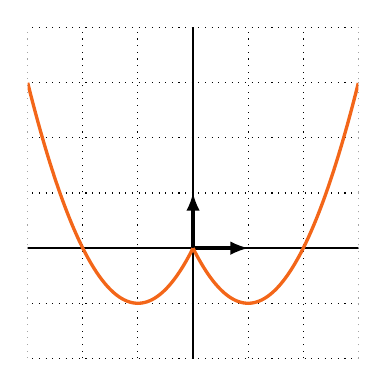
\begin{tikzpicture}[scale=0.7]
\clip (-3,-2) rectangle (3,4);
\draw [ thin, dotted] (-4,-2) grid (4,4);
\draw [thick] (-4,0)--(7,0);
\draw [thick] (0,-4) -- (0,5);
\draw [very thick,->,>=latex] (0,0)--(0,1);
\draw [very thick,->,>=latex] (0,0)--(1,0);
\draw [very thick, ocre,domain=-3:0,samples=100] plot (\x,{(\x+1)^2-1});
\draw [very thick, ocre,domain=0:3,samples=100] plot (\x,{(\x-1)^2-1});
\end{tikzpicture}
\end{center}

La fonction représentée ci-dessus est convexe sur $[-3;0]$ et sur $[0;3]$ mais n'est pas convexe sur $[-3,3]$.\end{example}


\section{Fonctions dérivables}

\subsection{Caractérisation des fonctions convexes}

\begin{proposition}Soit $f$ une fonction définie et dérivable sur un intervalle $I$. On note $\mathcal{C}_f$ la courbe représentative de $f$ dans un repère $\Oij$.
\begin{itemize}
\item $f$ est convexe sur $I$ si et seulement si la courbe $\mathcal{C}_f$ se trouve au-dessus de toutes ses tangentes aux points d'abscisses $x\in I$.
\item $f$ est concave sur $I$ si et seulement si la courbe $\mathcal{C}_f$ se trouve en-dessous de toutes ses tangentes aux points d'abscisses $x\in I$.
\end{itemize}\end{proposition}

\begin{minipage}{0.45\linewidth}
\begin{center}
\textbf{Fonction convexe}
\end{center}
\begin{center}
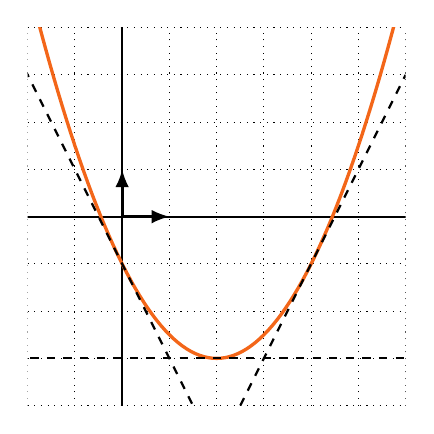
\begin{tikzpicture}[scale=0.6]
\clip (-2,-4) rectangle (6,4);
\draw [ thin, dotted] (-2,-4) grid (6,4);
\draw [thick] (-4,0)--(7,0);
\draw [thick] (0,-4) -- (0,5);
\draw [very thick,->,>=latex] (0,0)--(0,1);
\draw [very thick,->,>=latex] (0,0)--(1,0);
\draw [very thick, ocre,domain=-3:6,samples=100] plot (\x,{\x*\x/2-2*\x-1});
\draw [thick, dashed, domain=-3:6] plot (\x,2*\x-9);
\draw [thick, dashed,domain=-3:6] plot (\x,-3);
\draw [thick, dashed,domain=-3:6] plot (\x,-2*\x-1);

\end{tikzpicture}
\end{center}
\end{minipage}\hfill \begin{minipage}{0.45\linewidth}
\begin{center}
\textbf{Fonction concave}
\end{center}
\begin{center}
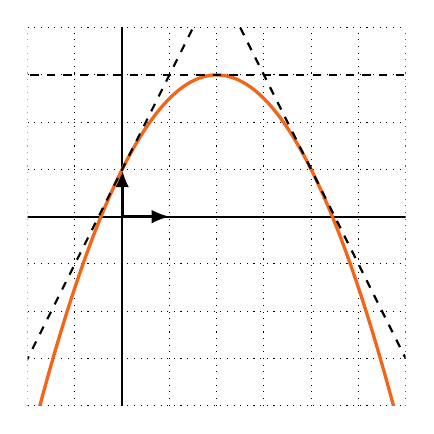
\begin{tikzpicture}[scale=0.6]
\clip (-2,-4) rectangle (6,4);
\draw [thin, dotted] (-2,-4) grid (6,4);
\draw [thick] (-4,0)--(7,0);
\draw [thick] (0,-4) -- (0,5);
\draw [very thick,->,>=latex] (0,0)--(0,1);
\draw [very thick,->,>=latex] (0,0)--(1,0);
\draw [very thick, ocre,domain=-3:6,samples=100] plot (\x,{-(\x*\x/2-2*\x-1)});
\draw [thick, dashed,domain=-3:6] plot (\x,-2*\x+9);
\draw [thick, dashed,domain=-3:6] plot (\x,3);
\draw [thick, dashed,domain=-3:6] plot (\x,2*\x+1);

\end{tikzpicture}
\end{center}
\end{minipage}

\begin{example} Montrons que la fonction $x\mapsto x^2$ est convexe sur $\mathbb{R}$. Notons $\mathcal{C}_f$ la courbe de $f$ dans un repère $\Oij$. Soit $a$ un réel.
\begin{itemize}
\item $f$ est dérivable sur $\mathbb{R}$ et pour tout réel $x$, $f'(x)=\qquad$.
\item La tangente à $\mathcal{C}_f$ a pour équation 
\newpage
\item Pour tout réel $x$, 
\[f(x)-(2ax-a^2)=\]
Ainsi, $\mathcal{C}_f$ est toujours au-dessus de sa tangente à l'abscisse $a$, et ce, peu importe le réel $a$ choisi. $f$ est donc convexe sur $\mathbb{R}$.
\end{itemize}\end{example}




\begin{proposition}Soit $f$ une fonction dérivable sur un intervalle $I$.
\begin{itemize}
\item $f$ est convexe sur $I$ si et seulement si $f'$ est croissante sur $I$.
\item $f$ est concave sur $I$ si et seulement si $f'$ est décroissante sur $I$.
\end{itemize}\end{proposition}

De cette propriété vient naturellement la suivante...

\begin{proposition}Soit $f$ une fonction deux fois dérivable sur un intervalle $I$.
\begin{itemize}
\item $f$ est convexe sur $I$ si et seulement si pour tout $x\in I$, $f''(x) \geqslant 0$.
\item $f$ est concave sur $I$ si et seulement si pour tout $x\in I$, $f''(x) \leqslant 0$. 
\end{itemize}
\end{proposition}

L'étude de la convexité d'une fonction revient à l'étude de signe de sa dérivée seconde (si celle-ci existe, bien entendu).

\begin{demonstration}\textbf{Si $f''\geqslant 0$, alors $f$ est convexe} : Soit $f$ une fonction deux fois dérivable sur $I$ telle que pour tout $x\in I$, $f''(x) \geqslant 0$.

\vskip200pt
\end{demonstration}
\newpage
\begin{example} Pour tout entier naturel pair $n\geqslant 2$, la fonction $x \mapsto x^n$ est convexe sur $\mathbb{R}$. \\ En effet, la dérivée seconde de cette fonction est la fonction $x\mapsto n(n-1)x^{n-2}$. \\Or, $n$ étant pair, $n-2$ l'est aussi, et pour tout réel $x$, on a donc $x^{n-2}\geqslant 0$.\end{example}

\begin{example}La fonction $f:x\mapsto x^3$ est concave sur $]-\infty ; 0]$ et convexe sur $[0;+\infty[$.

En effet, $f$ est deux fois dérivable sur $\mathbb{R}$ et pour tout réel $x$, $f''(x)=6x$, qui est positif si et seulement si $x$ l'est aussi.\end{example}

\subsection{Point d'inflexion}

\begin{definition}Soit $f$ une fonction dérivable sur un intervalle $I$.

Un \textit{point d'inflexion} est un point où la convexité de la fonction $f$ change. La tangente à la courbe de $f$ en un point d'inflexion traverse la courbe de $f$.\end{definition}

\begin{proposition}Soit $f$ une fonction deux fois dérivable sur un intervalle $I$. 
\begin{itemize}
\item Si $f$ présente un point d'inflexion à l'abscisse $a$, alors $f''(a)=0$.
\item Réciproquement, si $f''(a)=0$ et $f''$ \textbf{change de signe} en $a$, alors $f$ présente un point d'inflexion en $a$.
\end{itemize}\end{proposition}

Cela rappelle naturellement le cas des extremum locaux. Si $f$ admet un extremum local en $a$, alors $f'(a)=0$. Cependant, si $f'(a)=0$, $f$ admet un extremum local en $a$ seulement si $f'$ change de signe en $a$.

\begin{example}Pour tout réel $x$, on pose $f(x)=\dfrac{x^3}{2}-x+1$. 

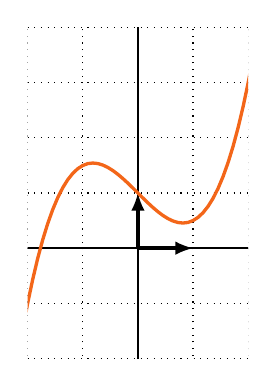
\begin{tikzpicture}[scale=0.7]
\clip (-2,-2) rectangle (2,4);
\draw [thin, dotted] (-2,-4) grid (6,6);
\draw [thick] (-4,0)--(7,0);
\draw [thick] (0,-4) -- (0,6);
\draw [very thick,->,>=latex] (0,0)--(0,1);
\draw [very thick,->,>=latex] (0,0)--(1,0);
\draw [very thick, ocre,domain=-3:6,samples=100] plot (\x,{\x*\x*\x/2-\x+1});

\end{tikzpicture}


\end{example}

\textbf{L'annulation de la dérivée seconde n'est pas une condition suffisante de présence d'un point d'inflexion !}


\begin{example}Pour tout réel $x$, on pose $g(x)=\dfrac{1}{12}x^4-\dfrac{2}{3}x^3+2x^2$. 

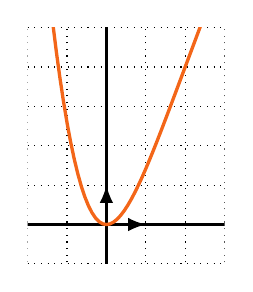
\begin{tikzpicture}[scale=0.5]
\clip (-2,-1) rectangle (3,5);
\draw [thin, dotted] (-2,-4) grid (6,6);
\draw [thick] (-4,0)--(7,0);
\draw [thick] (0,-4) -- (0,6);
\draw [very thick,->,>=latex] (0,0)--(0,1);
\draw [very thick,->,>=latex] (0,0)--(1,0);
\draw [very thick, ocre,domain=-3:6,samples=100] plot (\x,{\x^4/12-2*\x^3/3+2*\x*\x});

\end{tikzpicture}


\end{example}

\newpage
\section{Inégalités de convexité}

\subsection{Inégalités de milieux}


\begin{proposition}Soit $f$ une fonction convexe sur un intervalle $I$. 

Pour tous réels $a$ et $b$ de $I$, $ f\left( \dfrac{a+b}{2} \right) \leqslant \dfrac{f(a)+f(b)}{2}$.
\end{proposition}

\begin{demonstration}On considère les points $A(a,f(a))$ et $B(b,f(b))$. 


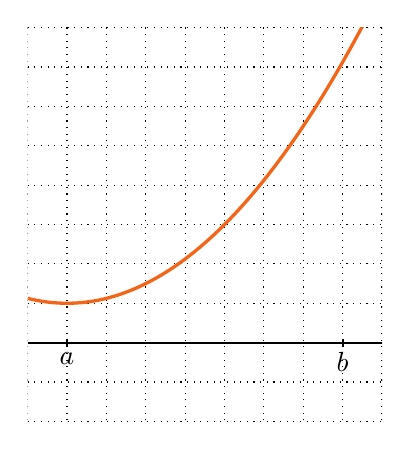
\begin{tikzpicture}[scale=0.5]
\clip (-6,-2) rectangle (3,8);
\draw [thin, dotted] (-6,-4) grid (6,9);
\draw [thick] (-6,0)--(7,0);
\draw [very thick, ocre,domain=-6:6,samples=100] plot (\x,{(\x+5)*(\x+5)/8+1});
\draw [thick] (-5,-0.1) -- (-5,0.1);
\draw (-5,0) node[below] {$a$};
\draw [thick] (2,-0.1) -- (2,0.1);
\draw (2,0) node[below] {$b$};



\end{tikzpicture}


\end{demonstration}

\begin{example}La fonction exponentielle est convexe sur $\mathbb{R}$. 

Pour tous réels $a$ et $b$,\end{example}

\begin{proposition}Soit $f$ une fonction concave sur un intervalle $I$. 

Pour tous réels $a$ et $b$ de $I$, $ f\left( \dfrac{a+b}{2} \right) \geqslant \dfrac{f(a)+f(b)}{2}$.
\end{proposition}

\begin{example}La fonction $x\mapsto \sqrt{x}$ est concave sur $\mathbb{R}_+$. 

Ainsi, pour tous réels $a$ et $b$ positifs,\end{example}

\subsection{Inégalités avec les tangentes}

La convexité des fonctions dérivables permet d'établir des inégalités en utilisant les équations des tangentes.

\begin{example}Montrons que pour tout réel $x$, $\e^x\geqslant x+1$.


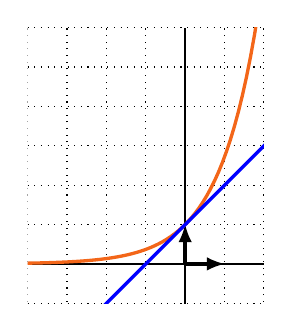
\begin{tikzpicture}[scale=0.5]
\clip (-4,-1) rectangle (2,6);
\draw [thin, dotted] (-4,-4) grid (6,6);
\draw [thick] (-4,0)--(7,0);
\draw [thick] (0,-4) -- (0,6);
\draw [very thick,->,>=latex] (0,0)--(0,1);
\draw [very thick,->,>=latex] (0,0)--(1,0);
\draw [very thick, ocre,domain=-4:6,samples=100] plot (\x,{exp(\x)});
\draw [very thick, blue,domain=-3:6,samples=100] plot (\x,1+\x);
\end{tikzpicture}



\end{example}







\end{document}